\section*{Network architecture}
\subsection*{MVSNet architecture}
\label{subsec:mvsnet}

\begin{figure*}[ht]
    \begin{center}
        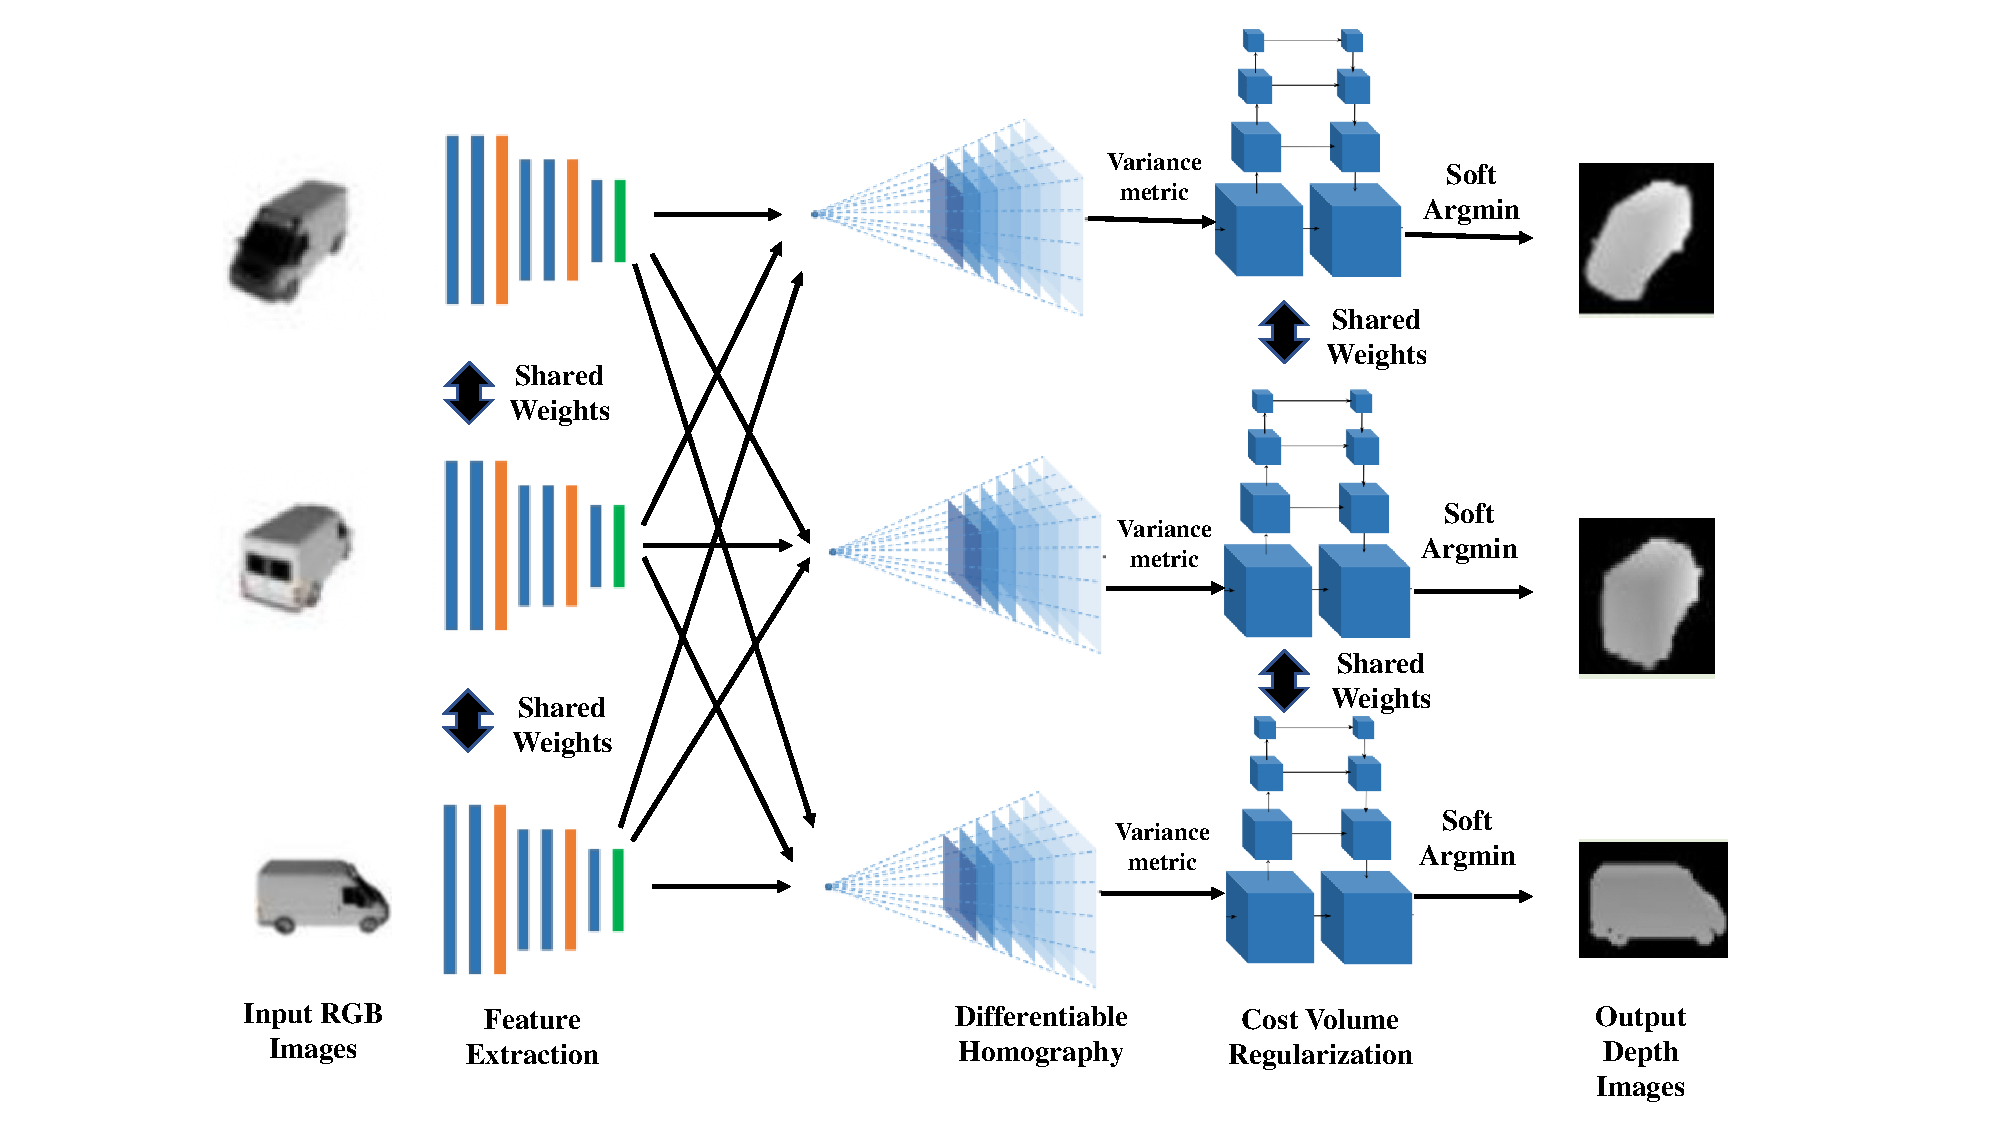
\includegraphics[width=\linewidth]{imgs/MVSNet_architecture.pdf}
    \end{center}
    \vspace{-4mm}
        \caption{Depth prediction network (MVSNet) architecture}
        \vspace{-4mm}
        \label{fig:mvsnet_architecture}
\end{figure*}

Our depth prediction module is based on MVSNet~\cite{yao2018mvsnet} which constructs a regularized 3D cost volumes
to estimate the depth map of the reference view.
Here, we extent MVSNet to predict the depth maps of all views instead of only the reference view.
This is achieved by transforming the feature volumes to each view's coordinate frame using homography warping
and applying identical cost volume regularization and depth regression on each view.
This allows the reuse of pre-regularization feature volumes for efficient multi-view depth prediction invariant to the order of input images.
\figref{mvsnet_architecture} shows the architecture of the our depth estimation module.

\subsection*{Probabilistic Occupancy Grid Merging}
We use single-view voxel prediction network from~\cite{gkioxari2019meshrcnn} to predict predicts voxel grids for each of the input images in their respective local coordinate frames.
The occupancy grids are transformed to global frame (which is set to the coordinate frame of the first image)
by finding the equivalent global grid values in the local grids after applying bilinear interpolation on the closest matches.
The voxel grids in global coordinates are then probabilistically merged according to~\subsecref{multiview_voxel} of the main submission.

